\documentclass[12pt]{article} %Define o documento como um artigo
\usepackage[portuguese]{babel} %Define a linguagem do documento como português
\usepackage[utf8]{inputenc} %Para entender todos os caracteres
\usepackage[a4paper, portrait, margin=2cm]{geometry} %Define a pagina como sendo tamanho A4, em modo retrato, com margem de 2 cm
\usepackage{dirtytalk} %Para usar o \say, que coloca aspas na frase
\usepackage{indentfirst} %Para indentar o primeiro parágrafo 
\setlength{\parindent}{2em} %Define o tamanho da indentação
\usepackage{soul} %Para fazer texto tachado
\usepackage{pgfplots} %Pacote de graficos
\pgfplotsset{compat=1.9}
\usepgfplotslibrary{statistics}
\usepackage{pgf-pie} %Graficos de pizza
\usepackage{wrapfig} %Figuras em volta de texto
\usepackage{tabularx} %Tabelas de qualquer tamanho
\usepackage{amsmath} %Biblioteca de integrais
\usepackage{mathtools} 
\usepackage{esint} %Biblioteca de integrais ciclicas
\usepackage{titlesec}
\usepackage{subcaption}
\usepackage{systeme}
\usepackage[spaces,hyphens]{url}
\usepackage{float}
\usepackage{subcaption}
\usepackage{multirow}
\usepackage{graphics}

\begin{document}

\begin{titlepage}
    \begin{center}
        
        \LARGE{\textbf{Métodos Numéricos e Aplicações - MAP3121}}
        
        \vspace{20pt}
        
        \LARGE{\textbf{Exercício-Programa 1}}
        
        \vspace{200pt}
        
        \LARGE{\textbf{Autovalores e Autovetores de Matrizes Tridiagonais Simétricas}}
        
        \vspace{40pt}
        
        \LARGE{\textbf{O Algoritmo QR}}
        
        \vspace{80pt}
        
        \begin{flushright}
            \Large{\textsc{Pedro H. G. Cazelatto - NUSP 11261090}}
        \end{flushright}
        
        \vfill
        
        São Paulo - SP
        
        01/07/2021
        
    \end{center}
\end{titlepage}

\section{Introdução}

    O programa foi desenvolvido em linguagem C para que sua execução fosse mais rápida. Para facilitar o entendimento inicial, realizei alguns \textit{scripts} no \textit{software} Octave conforme lia o enunciado, transformando o \say{matematiquês} em um código simples executável, o que ajudou no planejamento de funções, para minimizar repetição de código, e também na depuração do código final, pois me permitia conferir os valores.

    \vfill
    
\section{Primeiros Programas}
    
    Na primeira parte se deu a criação dos \textit{scripts} no Octave, simulando, conferindo valores e depurando quando algo ia para infinito. Precisei fazer isso pois fazer contas de matrizes em papel é muito trabalhoso, e o Octave oferece um degrau entre a simplicidade de um pseudocódigo e a complexidade de C, além de que me ajudou a entrar no ritmo para programar. Abaixo encontram-se os códigos que executam o algoritmo QR, sem e com o deslocamento espectral.
    
    \begin{figure}[H]
        \centering
        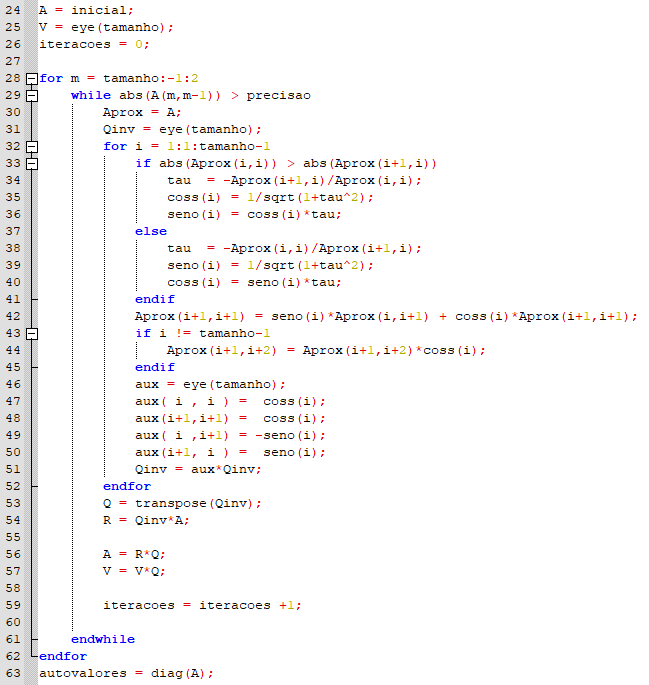
\includegraphics[width=0.75\linewidth]{QRsem.png}
        \caption{Algoritmo QR sem deslocamento espectral}
        \label{fig:QRsem}
    \end{figure}
    
    \begin{figure}[h]
        \centering
        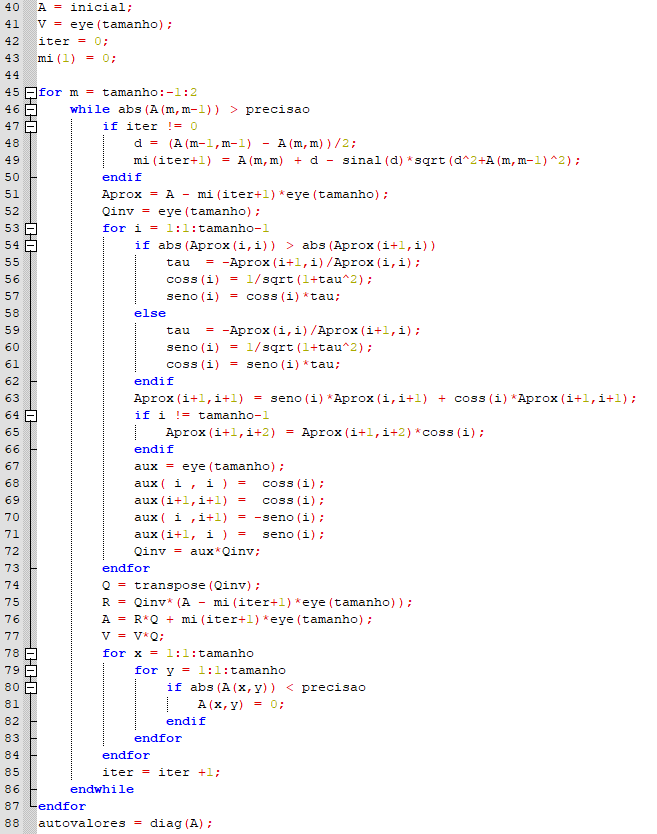
\includegraphics[width=0.75\linewidth]{QRcom.png}
        \caption{Algoritmo QR com deslocamento espectral}
        \label{fig:QRcom}
    \end{figure}
    
\section{Traduzindo para C}
    
    Após diversos testes bem sucedidos nos primeiros programas, comecei a separar funções que seriam necessárias para um funcionamento mais fluido do código, como somar, subtrair, multiplicar e transpor matrizes, que são a principal forma de dados. 
    
    O objetivo principal do EP é calcular a solução de um sistema massa-mola e sua evolução temporal através do algoritmo QR, para assim gerar gráficos da posição em função do tempo. Por isso, criei também uma função que gera a matriz de entrada\footnote{Matriz A descrita na página 8 do enunciado.} a partir das constantes elásticas de cada mola e da massa das massas, assim como duas funções que executam o algoritmo QR, uma com e outra sem deslocamento espectral, e devolvem os autovalores e autovetores associados a matriz de entrada. 
    
    A função \textit{main} é responsável por perguntar ao usuário qual teste ele deseja executar, pedir os parâmetros necessários para tal execução, imprimir na tela os dados iniciais do teste e seus resultados e coordenar as diversas funções já citadas de modo a executar o teste com perfeição.
    
\section{Testes}

    Junto com a descrição do problema e a explicação do algoritmo, alguns testes foram passado de modo a mostrar um uso real do código. 

    \subsection{Teste A}
    
        O primeiro dos testes serviu para mostrar a diferença que o deslocamento espectral, calculado a partir da heurística de Wilkinson, é capaz de promover no número de iterações necessárias para chegar na resposta aproximada.
        
        O teste é preparado usando como entrada uma matriz quadrada que contenha o número $2$ na diagonal principal e $-1$ na diagonal acima e abaixo da principal, fazendo com que o único parâmetro variável entre as execuções seja o tamanho da matriz. Abaixo, coloco uma tabela identificando o número de iterações para 4 tamanhos diferentes, com e sem o deslocamento espectral. A precisão do programa para a coleta dos dados foi de $\epsilon = 10^{-6}$, ou $0.000001$, como o programa pede. 
        
        \begin{table}[h]
            \centering
            \begin{tabular}{|c | c c c c c|} 
                \hline
                Tamanho da matriz & 4 & 8 & 16 & 32 & 64\\
                \hline\hline
                Sem deslocamento & 45 & 143 & 473 & 1600 & 5446\\ 
                \hline
                Com deslocamento & 7 & 15 & 31 & 59 & 109 \\
                \hline
            \end{tabular}
            \caption{Número de iterações do teste A}
            \label{tab:iterA}
        \end{table}
        
        Como é possível perceber, o deslocamento espectral ajuda muito na hora de fazer as contas, reduzindo drasticamente o número de iterações até a resposta aproximada.
        
        \begin{figure}[h]
            \centering
            \begin{subfigure}{0.475\linewidth}
                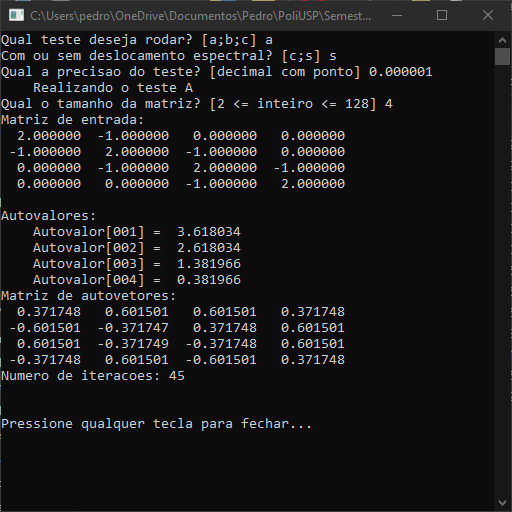
\includegraphics[width=\linewidth]{A4s.png} 
                \caption{Sem deslocamento}
                \label{fig:subA4s}
            \end{subfigure}
            \begin{subfigure}{0.475\linewidth}
                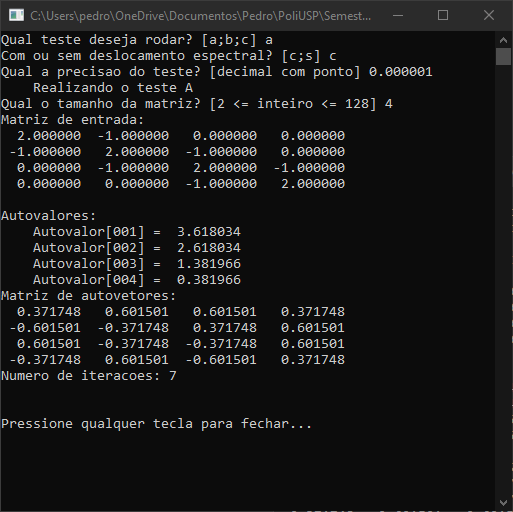
\includegraphics[width=\linewidth]{A4c.png}
                \caption{Com deslocamento}
                \label{fig:subA4c}
            \end{subfigure}
            \caption{Teste A com matriz 4 x 4}
            \label{fig:A4}
        \end{figure}
        
        \newpage
    
    \subsection{Teste B}
    
        Como segundo teste, foi pedido a solução temporal de um sistema massa-mola de 5 massas de 2 kg e 6 molas com constantes elásticas predefinidas sendo $k_i = (40+2i)$ N/m, $i = 1,...,6$, partindo de 3 conjuntos de posições iniciais diferentes e velocidade inicial nula. O programa calcula e salva em um arquivo de texto as posições de cada massa em função do tempo decorrido, permitindo-me gerar os gráficos abaixo.
        
        O primeiro conjunto de posições iniciais é $X_1(0) = [-2;-3;-1;-3;-1]$, o segundo é $X_2(0) = [1;10;-4;3;-2]$ e o terceiro é o modo de maior frequência. As frequências de oscilação são iguais a raiz quadrada dos autovalores da matriz de entrada, enquanto o modo de vibração associado àquela frequência é o autovetor associado ao autovalor correspondente.
        
        \begin{table}[h]
            \centering
            \begin{tabular}{|c|c|c|c|c|c|} 
                \hline
                Frequência (rad/s) &  9,405 &  8,373 &  6,839 &  4,837 &  2,504 \\
                \hline\hline
                                   &  0,189 &  0,475 &  0,599 &  0,533 &  0,310 \\ 
                                   & -0,391 & -0,585 & -0,103 &  0,474 &  0,518 \\
                Modos de vibração  &  0,558 &  0,185 & -0,565 & -0,064 &  0,576 \\
                                   & -0,588 &  0,383 &  0,093 & -0,517 &  0,481 \\
                                   &  0,393 & -0,501 &  0,551 & -0,469 &  0,269 \\
                \hline
            \end{tabular}
            \caption{Frequências e modos de vibração do teste B}
            \label{tab:freqB}
        \end{table}
        
        Como é possível ver na figura \ref{fig:B3}, quando a posição inicial das massas é um múltiplo dos modos de vibração, que no meu caso é 1, as massas se movem com a mesma frequência associada ao modo, que no caso do teste 3 é a maior das frequências, $9,405$ rad/s ou $1,497$ Hz. 
    
        \begin{figure}[H]
            \centering
            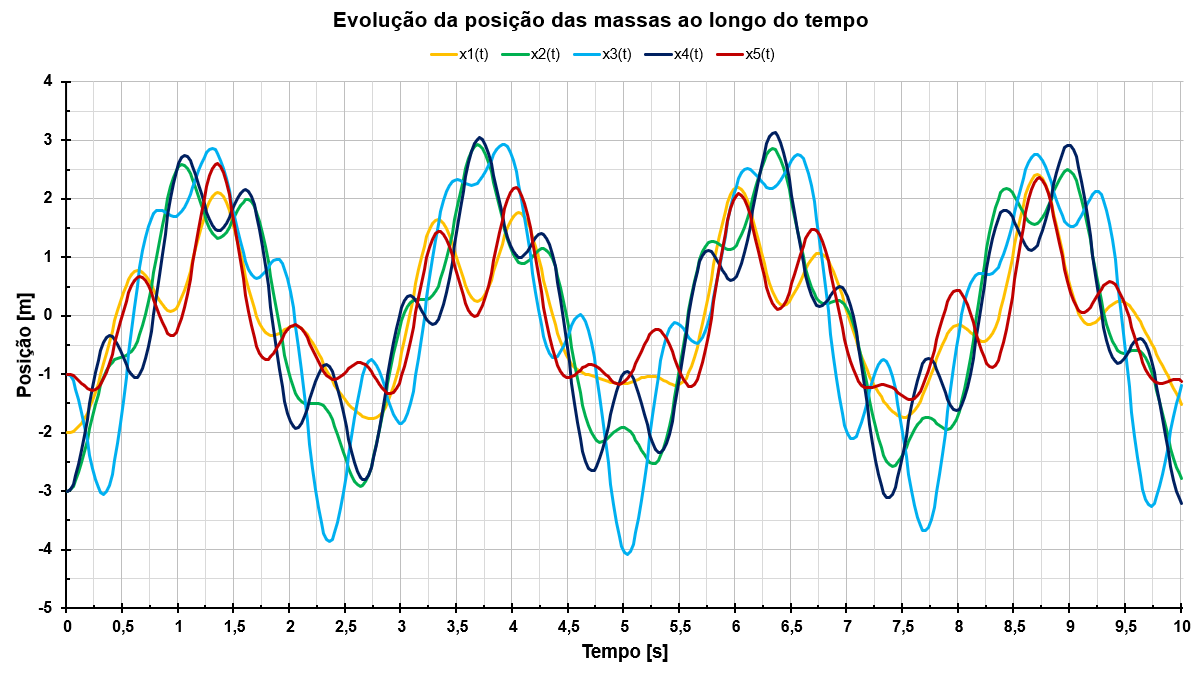
\includegraphics[width=0.95\linewidth]{B1.png}
            \caption{Teste B1}
            \label{fig:B1}
        \end{figure}
        
        \begin{figure}[H]
            \centering
            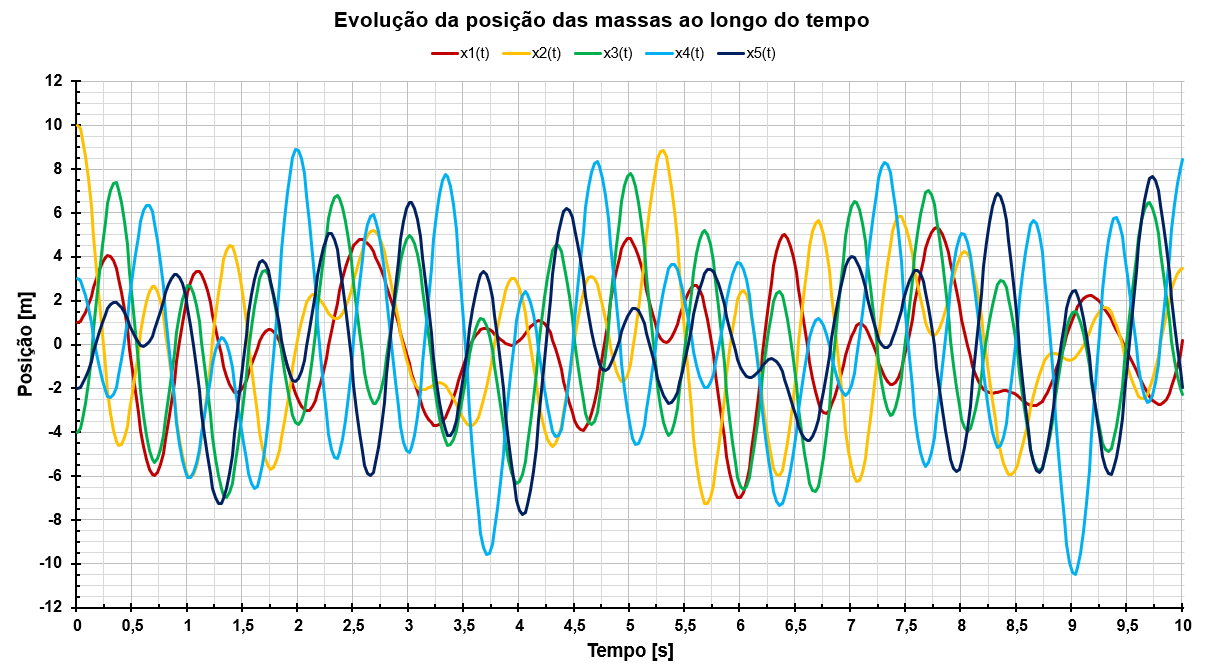
\includegraphics[width=0.95\linewidth]{B2.png}
            \caption{Teste B2}
            \label{fig:B2}
        \end{figure}
        
        \begin{figure}[H]
            \centering
            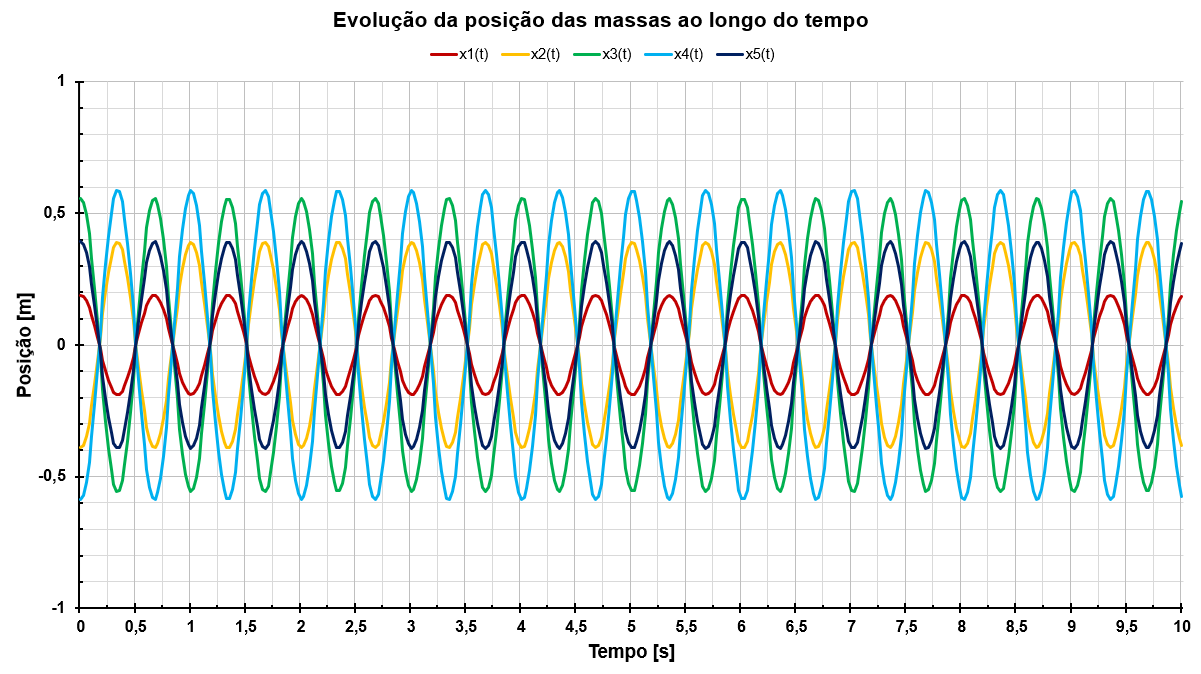
\includegraphics[width=0.95\linewidth]{B3.png}
            \caption{Teste B3}
            \label{fig:B3}
        \end{figure}
        
        \newpage
    
    \subsection{Teste C}
    
        Para o terceiro teste, foi pedida a solução temporal de um sistema massa-mola mais complexo do que o teste B, com 10 massas de 2 kg e 11 molas de constantes elásticas predefinidas sendo $k_i = (40+2(-1)^i)$ N/m, $i = 1,...,6$, partindo dos mesmos 3 conjuntos de posições iniciais do teste B, repetindo os valores nas posições 6 a 10, e velocidade inicial nula.
        
        Da mesma maneira, o programa calcula e salva em um arquivo de texto as posições de cada massa ao longo do tempo. Como também é possível ver na figura \ref{fig:C3}, quando as massas começaram na posição indicada pelo autovetor associado ao maior autovalor, todas oscilaram com frequência $8,854$ rad/s, ou $1,409$ Hz.
        
        \begin{table}[H]
            \centering
            \resizebox{\columnwidth}{!}{
            \begin{tabular}{|c|c|c|c|c|c|c|c|c|c|c|} 
                \hline
                Frequência (rad/s) & 8,854 & 8,587 & 8,148 & 7,554 & 6,856 & 5,744 & 4,789 & 3,689 & 2,504 & 1,265 \\
                \hline\hline
                         &  0,125 &  0,240 &  0,335 &  0,398 &  0,395 &  0,395 &  0,398 &  0,335 &  0,240 &  0,125 \\ 
                         & -0,229 & -0,386 & -0,420 & -0,324 & -0,132 &  0,132 &  0,324 &  0,420 &  0,386 &  0,229 \\
                         &  0,324 &  0,419 &  0,214 & -0,150 & -0,388 & -0,388 & -0,150 &  0,214 &  0,419 &  0,324 \\
                         & -0,386 & -0,324 &  0,111 &  0,414 &  0,249 & -0,249 & -0,414 & -0,111 &  0,324 &  0,386 \\
                Modos de &  0,421 &  0,113 & -0,391 & -0,207 &  0,337 &  0,337 & -0,207 & -0,391 &  0,113 &  0,421 \\
                vibração & -0,421 &  0,113 &  0,391 & -0,207 & -0,337 &  0,337 &  0,207 & -0,391 & -0,113 &  0,421 \\
                         &  0,386 & -0,324 & -0,111 &  0,414 & -0,249 & -0,249 &  0,414 & -0,111 & -0,324 &  0,386 \\
                         & -0,324 &  0,419 & -0,214 & -0,150 &  0,388 & -0,388 &  0,150 &  0,214 & -0,419 &  0,324 \\
                         &  0,229 & -0,386 &  0,420 & -0,324 &  0,132 &  0,132 & -0,324 &  0,420 & -0,386 &  0,229 \\
                         & -0,125 &  0,240 & -0,335 &  0,398 & -0,395 &  0,395 & -0,398 &  0,335 & -0,240 &  0,125 \\
                \hline
            \end{tabular}
            }
            \caption{Frequências e modos de vibração do teste C}
            \label{tab:FreqC}
        \end{table}
    
        \begin{figure}[H]
            \centering
            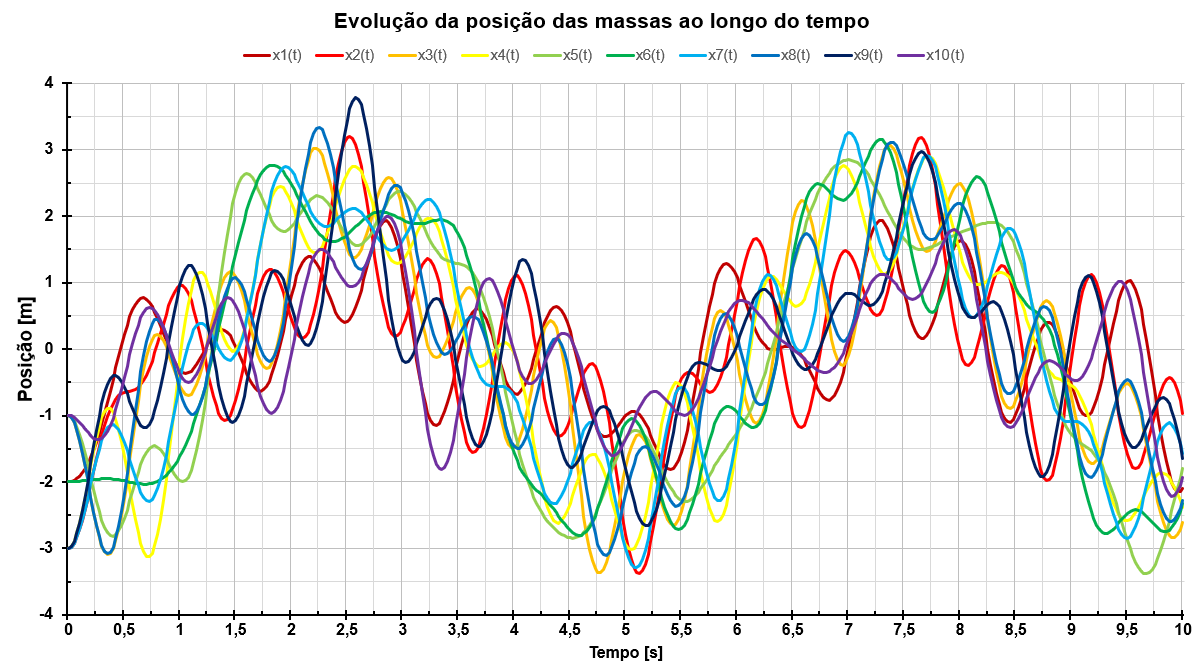
\includegraphics[width=0.95\linewidth]{C1.png}
            \caption{Teste C1}
            \label{fig:C1}
        \end{figure}
        
        \begin{figure}[H]
            \centering
            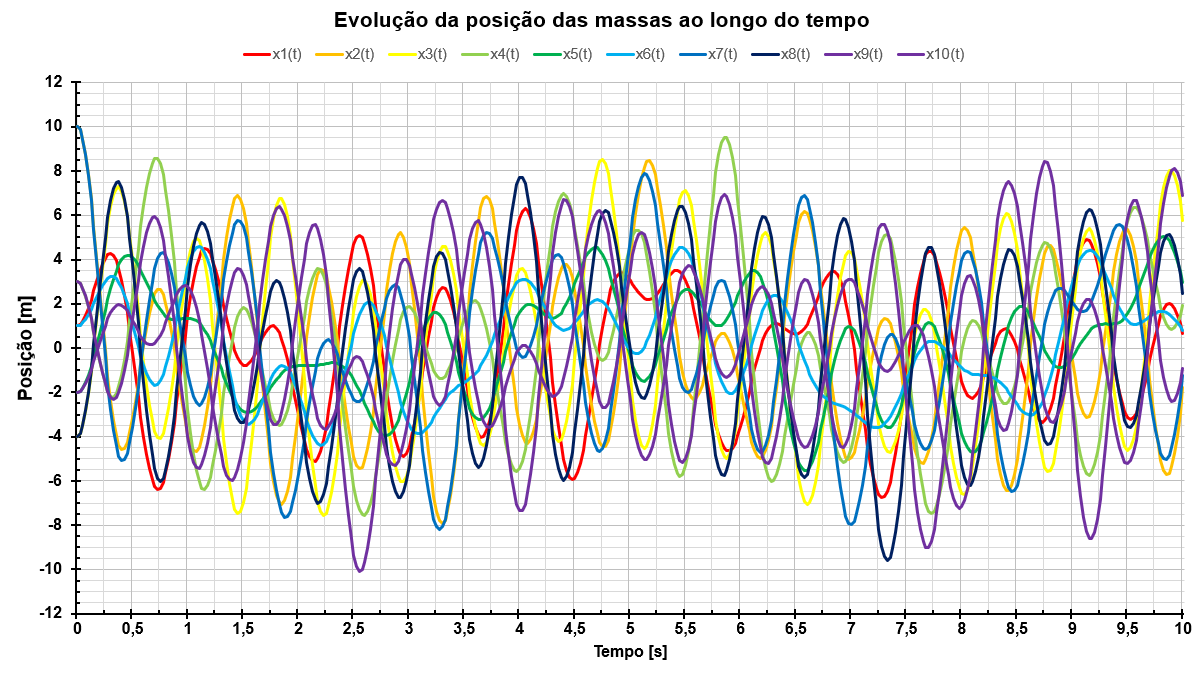
\includegraphics[width=0.95\linewidth]{C2.png}
            \caption{Teste C2}
            \label{fig:C2}
        \end{figure}
        
        \begin{figure}[H]
            \centering
            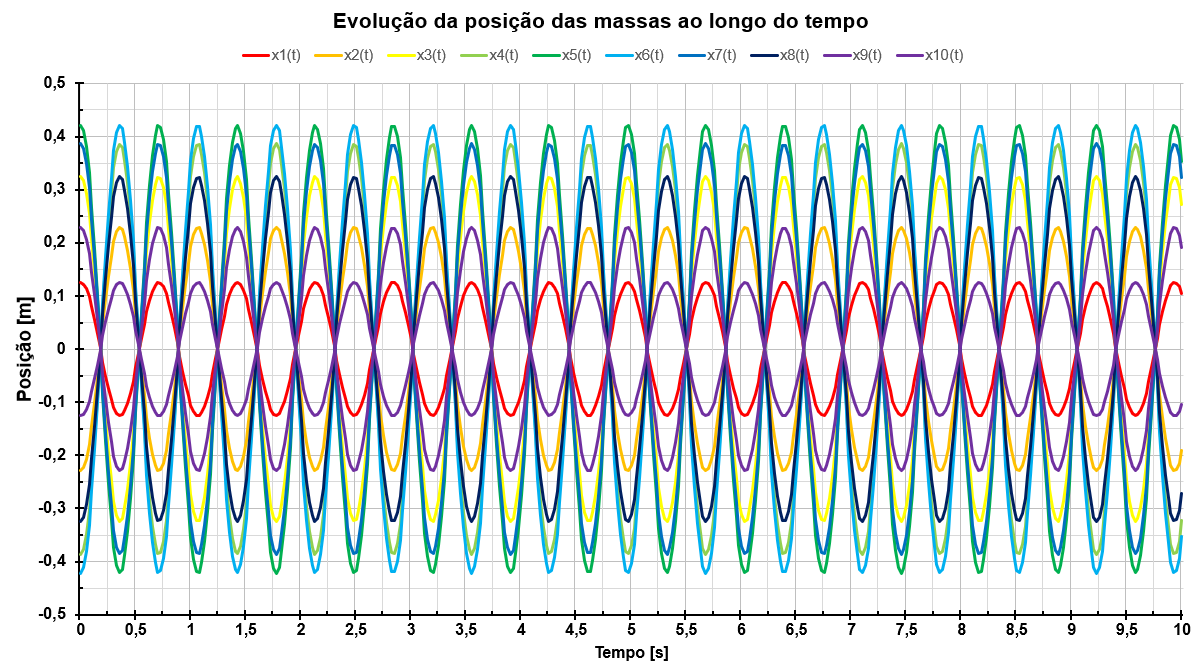
\includegraphics[width=0.95\linewidth]{C3.png}
            \caption{Teste C3}
            \label{fig:C3}
        \end{figure}



\end{document}